\begin{figure}[h]
\centering 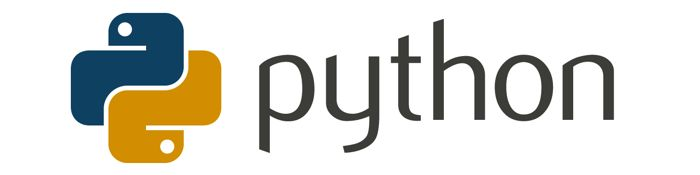
\includegraphics[scale=0.3]{images/python.jpg}
\end{figure}
\noindent Python is a dynamic language, as in python coding is very easy and 
also it require less coding and about its interpreted nature it is 
just exellent. Python is a high level programming language and Django 
which is a web development framework is written in python language.

Python is an easy to learn, powerful programming language.Python runs 
on Windows, Linux/Unix, Mac OS X. Python is free to use, even for 
commercial products. Python can also be used as an extension language 
for existing modules and applications that need a programmable interface.  
Python is free to use, even for commercial products, because of its 
OSI-approved open source license.
\subsection{Features of Python}
\begin{itemize}
\item Very clear, readable syntax.
\item Strong introspection capabilities.
\item Intuitive object orientation.
\item Natural expression of procedural code.
\item Full modularity, supporting hierarchical packages.
\item Exception-based error handling.
\item Very high level dynamic data types.
\item Extensive standard libraries and third party modules for virtually every task.
\item Extensions and modules easily written in C, C++ (or Java for Jython, or .NET languages for IronPython).
\item Embeddable within applications as a scripting interface.
\end{itemize}
\subsection{Installation of Python}
Installation of python is a very easy proccess.
The current python versions are: Python 2.7.1 and Python 3.2.
Type the commands in the terminal:\\

 \$ wget http://www.python.org/ftp/python/2.7/Python-2.7.tgz\\

 
 \$ tar xzf Python-2.7.tgz\\


This will install the python on your pc/laptop.

